
Throughout, we use $\Theta$ to refer to some space of possible belief states,
and $\Phi$ for a set of possible inputs. 
\commentout{% have now already given these examples more clearly; now cut to the chase!
	For example, a belief state $\theta \in \Theta$
	might be probability distribution,
	a Dempster-Shafer belief function, or
	weights for a neural network,
	while an input $\phi \in \Phi$ might be an event, or a sample from a dataset. 
}
%
% $\Theta$ might be \textellipsis
% \begin{itemize}[nosep]
%     \item $\Delta W$, the set of probability distributions over measurable space $W$ of outcomes;
%     \item the set of parameters to some parametric family of distributions;
%     \item the set of belief functions over a common space of outcomes;
%     \item the set of all possible PDGs;
%     \item a set of worlds an agent considers possible;
%     \item
% % \end{itemize}
Now, suppose we have some initial belief state $\theta$, and observe $\phi$ with confidence $\alpha \in [0,1]$. 
How do our beliefs change as a result? 
To study this mathematically, we assume that the process can be captured in functional form:
\unskip\footnote{%
	% we can just as easily handle randomized updates;
	It should be straightforward to extend our theory
	so as to handle randomized updates as well;
	the point is that
	% the update can be prescribed by an algorithm.
	the belief state, observation, and confidence must together contain
	enough information to describe the updating process.
	}
\begin{CFaxioms}
	\setcounter{CFaxiomsi}{-1}
	\item
	% \item[CF0]
	There exists some function
	$
	% \[
		% F : \confdom \to ( \Phi \to ( \Theta \to \Theta) )
		F :  \Phi \times [0,1] \times \Theta \to \Theta
	% \]
	$
	which, given input $\phi \in \Phi$, confidence $\chi \in [0,1]$, and a prior belief state $\theta \in \Theta$, 
	produces the appropriate posterior belief state $F(\phi, \chi, \theta) \in \Theta$. 
	 % belief state $F^c_\phi\theta$ that corresponds to the result of observing $\phi$ in state $\theta$. 
	 	\label[CFaxiomsi]{ax:funcform}
\end{CFaxioms}

Given such a function $F$, as well as a statement $\phi \in \Phi$
and confidnece $\chi \in [0,1]$, we call 
$F^\chi_\phi = F(\phi, \chi, -) : \Theta \to \Theta$
% a (confidence-$\chi$) \emph{update}.
an \emph{update}.
To ensure $F$ captures the belief updating process, we also require that it satisfy some axioms, characterizing the important shared features between \cref{ex:prob-simple,ex:classifier,ex:shafer}.
First, we would like no-confidence updates to leave our belief state unchanged. 

\begin{CFaxioms}
	% \item \textbf{(zero)} $F^{0}_A(\Pr) = (\Pr)$
	% \item  $F^{0}_A  = {1}_{\Delta\X}$. (That is, $F^{0}_A(\Pr) = \Pr$ for all $\Pr \in \Delta\X$.)
	% \item  $F^{0}_\phi  = {1}_{\Delta\X}$. (That is, $F^{0}_\phi(\Pr) = \Pr$ for all $\Pr \in \Delta\X$.)
	%     \hfill \textbf{(zero)} \label{ax:zero}
	\item
		% $F^{\bot}_\phi  = {\mathrm{Id}}_{\Theta}$.\\
		% (That is, $F^{\bot}_\phi(\theta) = \theta$ for all $\theta \in \Theta$.)
		% For all $\theta \in \Theta$ and $\phi \in \Phi$, $F^{\bot}_\phi(\theta) = \theta$.
		% No-confidence updates are identities. 
		% That is,
		For all $\theta \in \Theta$ and $\phi \in \Phi$,
		 $F^{0}_\phi(\theta) = \theta$.
		% \hfill \textbf{(no-confidence)} 
		% \hfill \textbf{(no-conf)} 
		% \hfill \textbf{(zero)} 
		% \hfill \textbf{(neutrality)} 
		\label{ax:zero}
\end{CFaxioms}


% Thus, a no-confidence update simply discares the new observation.
% At the opposite extreme, we call $F^1_\phi$ a \emph{full update}. 
% The appropriate way to deal with full confidence depends
% At the opposite extreme, the appropriate way to deal with full confidence
The appropriate way to deal with full confidence, on the other hand,
depends on the relationship between $\Theta$ and $\Phi$,
but it still characterized by an important property.
% , but it can still be characterized at this level of generality.


% \textbf{High Confidence Updates.}
\subsection{Updating with Full Confidence}
Since the purpose of $F^1_\phi$ is to \emph{fully} incorporate $\phi$ into our beliefs,
two successive updates with the same information ought to have the same effect as a single one.
Intuitively, this is because if we have just updated our beliefs to be consistent with the information $\phi$, then a second observation of $\phi$ will require no further alterations of our belief state.
% In this case, we call $F$ an \emph{update rule}, or more precisely, a \emph{$\Theta$-update rule on $\Phi$}, and insist that

\begin{defn}
	A \emph{full-confidence ($\Theta$-)update rule} (for $\Phi$) is
	a mapping $P: \Phi \times \Theta \to \Theta$ such that
	for all $\phi \in \Phi$, 
	$P_\phi = (\theta \mapsto P(\phi,\theta)): \Theta \to \Theta$ is idempotent.
	That is,	
	$P_\phi(P_\phi(\theta)) = P_\phi(\theta)$
	 for all $\phi\in\Phi$ and $\theta \in \Theta$.
\end{defn}

\begin{CFaxioms}
	\item
	% Full-confidence updates are idempotent.
	% For all $\phi \in \Phi$, the update $F_\phi$ is idempotent.
    % That is, for all $\phi \in \Phi$,  $F^1_\phi \circ F^1_\phi = F^1_\phi$.
    % That is, for all $\phi \in \Phi$ and $\theta \in \Theta$,  $F^1_\phi \circ F^1_\phi = F^1_\phi$.
    % (i.e., $F^1_\phi \circ F^1_\phi = F_\phi$).
	Full-confidence updates are idempotent. Or,
	equivalently,
	$F^1 = (\phi, \theta) \mapsto F(\phi,1,\theta): \Phi \times \Theta \to \Theta$ is a full-confidence
	update rule.
	\label{ax:idemp}
\end{CFaxioms}



% In curried form, $F : \Phi \to (\Theta \to \Theta)$.

% We now proceed with the formal details.
% \textbf{Update Rules.}
% Consider a space $\Theta$
% of possible belief states,
% and a set $\Phi$ of statements.
% % and a set $\Phi$ of ``statements'', i.e., the things one can have confidence in.
% % An \emph{update rule} (or more precisely, a \emph{$\Theta$-updating rule on $\Phi$})
% An \emph{update rule}, or more precisely, a \emph{$\Theta$-update rule on $\Phi$},
% is a function of the form
% \[
%     % F :  (\mathbb R \times \Phi) \to \Big( \Theta \to \Theta \Big)
%     F :  \Phi \to \Big( \Theta \to \Theta \Big)
% \]
% % which describes how to update beliefs about $X$, with the new information, at a certain level of trust.
% which describes how to (fully) update beliefs $\Theta$ with new information $\Phi$.
% and for $F$ to be an update rule, we require that , meaning that updating any belief with $\phi$ twice in a row is equivalent to single update.
% Having said that, one reading of this paper is a relaxation of this requirement.
% Here are some examples.
Once $\Theta$, $\Phi$, and any implicit structure in them is specified, there is often a natural choice of full-confidence update rule.
To illustrate, we now consider three different rules for different choices of $\Phi$.
In each case, the possible belief states $\Theta := \Delta W$ be the set of all probability distributions over a finie set $W = \{w_1, \ldots, w_n\}$ of ``possible worlds''.

\begin{enumerate}[wide, label=\textbf{\thesubsection.\arabic*}]
	\item %\textbf{Conditioning.}
	\textbf{Conditioning.}
	First, consider the case where observations are events, i.e., $\Phi := 2^W$.
	% One particularly natural $\Delta W$-update rule on $2^W$ is given by conditioning,
	% Here, the appropriate update seems to be condition:
	Here, the appropriate rule seems to be conditioning:
	% \[
	% \begin{aligned}
	% 	(-) \smash{\,\Big|\,} (\;\cdot\;) : \qquad 2^W &\to (\Delta W \to \Delta W) \\
	% 	A  &\mapsto (  ~\mu~~ \mapsto \mu \mid A ~),
	% \end{aligned}
	% \]
	% where $(\mu \mid A)(x) = \frac{\mu(\{x\})}{\mu(A)}$
	% in which learning $A$ maps
	% where the action of the conditional measure $\mu\mid A$ is given by $(\mu \mid A) \{w\} = \ifrac{\mu\{w\}}{\mu(A)}$.
	% where the action of the conditional measure $\mu\mid A$ is given by $(\mu \mid A)(B) = \ifrac{\mu(B \cap A)}{\mu(A)}$, provided $\mu(A) > 0$,
	starting with $\mu \in \Delta W$, the conditional measure 
	$\mu\mid A$ is given by $(\mu \mid A)(B) = \ifrac{\mu(B \cap A)}{\mu(A)}$, provided $\mu(A) > 0$,
	% and may be defined arbitrarily otherwise.
	and otherwise is just equal to $\mu$.
	Observe:
	\begin{itemize}[nosep, leftmargin=1.2em]
		\item Provided $\mu(A) > 0$, then $(\mu\mid A) \mid A = \mu \mid A$, so conditioning is a full-confidence update.
		\item If $\mu(A \cap B) > 0$, then $(\mu \mid A) \mid B = \mu \mid (A \cap B) = (\mu \mid B) \mid A$, so the order that information is recieved does not matter (so long as it is consistent with one's beliefs).
	\end{itemize}
	There are well-known issues with conditioning $\mu$ on $A$ when
	$\mu(A) = 0$, typically this operation is undefined. Note that to satisfy
	\cref{ax:idemp}, the result must either be $\mu$ itself or a
	 distribution that gives probability 1 to $A$. 
	% However, it is not the only $\Delta W$-updating rule for $2^W$.
	 % $\Phi$.

	\item
	\textbf{Imaging.}
	A second example of an update rule is the ``imaging'' approach of David Lewis
	\parencite{lewis1976probabilities}.
	% , albeit in very different notation.
	% Once again, consider a finite set $W$, and belief states $\Theta := \Delta W$.
	Suppose that, for some set $\Phi$, that we already have a full-confidence update rule
	$f : \Phi \times W \to W$ on individual worlds, which we interperet as assigning each statement $\phi \in \Phi$ and $w \in W$ an element $f(\phi, w) \in W$ which is the unique ``world most similar to $w$, in which $\phi$ is true'' \parencite{gardenfors1979imaging}.
	In this case, idempotence of $f_\phi: W \to W$ amounts to the (very reasonable) requirement that the world most similar to $f_\phi w$ in which $\phi$ is true, is $f_\phi w$ itself.
	From $f$, we can construct a full confidence update rule $F$ for $\Delta W$
	with the pushforward	
	\[
    	\begin{aligned}
    		% F_\phi(\mu) &:=
    		F(\phi, \mu) 
				% &:=
				% f^{\sharp}(\mu)
    			% &= A \mapsto \mu( f^{-1}_\phi( A ))\\
    			&= A \mapsto \mu(\{w : f(w, \phi) \in A\})
    	\end{aligned}
		% \qquad
		% \qquad
		% \begin{tikzpicture}[center base]
		% 	\node[dpad0] (W) {$W$};
		% 	\node[dpad0, right=1 of W] (W') {$W$};
		% 	\node[dpad0, below right=0.2 and 0.2 of W] (Phi) {$\Phi$};
		% 	\mergearr{W}{Phi}{W'}
		% 	\node[above=1pt of center-WPhiW']{$f$};
		% 	\draw[arr2, <-] (W) to node[above]{$\mu$} ++(-1, 0);
		% 	\draw[arr2, <<-] (Phi) to node[below]{$\phi$} ++(-1.3, 0);
		% 	\draw[arr2, <-, dashed, gray] (W') to node[above]{$F_\phi(\mu)$} ++(2, 0);
		% \end{tikzpicture}
	\]
	which intuitively moves the probability mass on each world $w$ to the $f_\phi w$, the closest world to $w$ in which $\phi$ is true.
	% is the pushforward measure of $\mu$ through $f_\phi$, which Lewis calls the ``image of $\mu$ on $\phi$''
	And, since $f$ is idempotent, $F$ will be as well.


	\commentout{
	\item More generally, consider a measurable space $\mathcal W = (W, \mathcal A)$, where $W$ is a set and $\mathcal A$ is a $\sigma$-algebra over $W$, and let $\mathcal F \subset \mathcal A$ be closed under supersets in $\mathcal A$.
	% Now, let $\Theta$ be the set of conditional probabili$

	\TODO[Properly Use Conditional Probability Measure, to define on all events]

	Conditioning a probability distribution $\mu \in \Delta\X$ on an event $A \in \mathcal A$ also makes sense in this more general measure-theoretic setting, at least so long as $\mu(A) > 0$, and is given by
	% the Lebesgue integral
	% \[
	$$
		% (\mu \mid A) (B) = \frac{1}{\mu(A)} \int \mathbf 1_{B}(x)  \mathrm d\mu(x)
		(\mu \mid A) (B) = \frac{\mu(B \cap A)}{\mu(A)}
	$$
	}


	\item
	\textbf{Jeffrey's Rule.}
	% Once more, suppose that $W$ is a finite set and $\Theta := \Delta W$.
	Next, consider a more general form of observation, in which observations themselves are probabilities.
	% Formally, suppose $\Phi$ consists of pairs $(X,\pi)$,
	Formally, let $\Phi$ be the set of pairs $(X,\pi)$,
	% Formally, suppose $\Phi$ consists of marginal distributions $\pi(X)$
	% Formally, suppose $\Phi$ consists of distributions $\pi(X)$,
	% written $\pi(X)$,
	where $X : W \to S$ is a random variable taking values in some set $S$,
	% (i.e., some function of $W$),
	and $\pi \in \Delta S$ is a probability on
	% the possible values that $X$ can take.
	$S$.
	Jeffrey's rule is then:
	\begin{align*}
		% \mathrm{Jeffrey}_{(X,\pi)}
		% \mathrm{Jeffrey}_{\pi(X)}
		% \mathrm{J}_{\pi(\mskip-2muX\mskip-2mu)}
		\mathrm{J}_{(X,\pi)}
		(\mu) &:= \sum_{x \in S} \pi(X{=}x) \;  \mu \big|
            (X{=}x)
            % \{ w : X(w) = x \}
			% \\
			% &= A \mapsto \sum_{x \in S} \pi(X{=}x)\, \mu( A \mid X \!= x)
	\end{align*}

	When $\pi$ places all mass on some $x \in S$, Jeffrey's Rule amounts to conditioning on $X {=} x$.
	 % but for other choices of $\pi(X)$,
	For this reason, Jeffrey's Rule is sometimes often thought of as a generalization of conditioning that admits for less that complete certainty.
	However, it is still a full-confidence update rule---just one that handles observations that can be uncertain.

	Let $\mu' := J_{\pi(X)}(\mu)$ be the result of applying Jeffrey's rule for $(X,\pi)$ to $\mu$.
	% then $\pi$ will be fully incorporated (that is, $\mu'(X) = \pi(X)$),
	Note that $\mu'(X) = \pi(X)$, so $\pi(X)$ has been fully incorporated into $\mu'$, while all information about the old prior belief about $X$ has been destroyed by the update.
\end{enumerate}


\subsection{%
	% Continuity and
 	The Path of Middling Confidence}

Full updates are quite extreme.
An agent that updates by conditioning, for instance,
% is permanently commited to believing everything it ever learns with perfect certainty,
permanently commits to believing everything it ever learns,
and gains nothing from making the same observation twice.
 % (\cref{ax:idemp})
% Humans don't work this way. The effectiveness of flash cards as a learning tool demonstrates this clearly: if we were using an update rule, two cycles through a deck of flash cards would be no different from one.
Clearly humans are not like this; revisiting information
 	improves our learning \parencite{ausubel1965effect}.
Similarly, artificial neural networks are trained with
 	many incremental updates, and benefit from seeing 
	the training data many times.
% Indeed, this is one biggest differences between modern machine learning techniques and  older rule-based ones: modern algorithms update parameters little-by-little, rather than fully incorporating input information.
% Once an agent that uses conditioning incorporates $A$, it is forever committed to believing $A$, and as a side effect, there is no point to making
We would like an account that allows for for less extreme belief alterations,
in which information is only partially incorporated.
This is the role of intermediate values of confidence.

Since confidence is supposed to interpolate between prior beliefs and full update,
we would like each $\chi \mapsto F(\theta,\chi,\phi) : [0,1] \to \Theta$
to be a continuous path in belief states, from the initial belief to full incorporation.

\begin{CFaxioms}[nosep]
	\item
	$\Theta$ comes with a topology, with respect to which
	the restriction
	$F_{\phi}|_\theta : [0,1] \to \Theta$
	is continuous
		% for all $\phi, \theta \in \Phi\times\Theta$.
	for all $\phi \in \Phi$ and $\theta \in \Theta$.
	\label{ax:cont}
\end{CFaxioms}


% For this to be meaningful, we need $\Theta$ to be a topological space,
% in which case the simplest and most convenient thing would be to require:

It would be particularly nice if updates were continuous in our initial
beliefs as well: after all, similar priors typically result
in similar posteriors beliefs. This would allow us to strengthen
\cref{ax:cont} to something simpler:

\begin{CFaxioms}[nosep]
	\item
	% [TOP]
	% [CF{\the\numexpr\value{CFaxiomsi}+1\relax}${^\prime}$]
	[CF{\the\numexpr\value{CFaxiomsi}\relax}${^\prime}$]
	% $\Theta$ is a topological space, and
	$\Theta$ comes with a topology, with respect to which
	% \item
	$F_\phi : [0,1] \times \Theta \to \Theta$ is continuous
	for all $\phi \in \Phi$.
	\label{ax:cont-strong}
\end{CFaxioms}

Unfortunately, this is too strong to handle extreme beliefs.
In the probabilistic case, for instance:

% Axiom \cref{ax:cont-strong} says more---it says that the posterior 
% belief is also continuous in the prior beliefs, 
% which also seems appropriate. But this assumption has significant bite.

% \commentout{%
% actually, this shows a problem with defining 
%
% \begin{example}
% 	Again let $W$ be a finite set, and choose disjoint non-empty subsets
% 	$A, B \subset W$ with $A \cap B = \emptyset$.
% 	Let $p\ne q$ be two distinct distributions over $W$ supported
% 	on $A$, and $d$ be one suppoerted on $B$. Now, consider 
% 	% and consider a sequence $(\mu_i)_{i \in \mathbb N}$ of positive probability 
% 	% distributions over $W$ whose limit 
% 	% is the point mass $\delta_w$ on a particular world $w \in W$.
% 	% $\mu^*$ has support $A \subsetneq W$ (i.e., $\mu^*(A)=1$).
% 	the two sequences of probability distributions
% 	\[
% 		\Big(p_n= (1-e^{-n}) d + (e^{-n}) p \Big)_{n \in \mathbb N}
% 		,
% 		\qquad
% 		\Big(q_n = (1-e^{-n}) d + (e^{-n}) q \Big)_{n \in \mathbb N},
% 	\]
% 	both of which have limit $d$. But every $p_n | A = p$ while every $q_n |A = q$, so
% 	now \cref{ax:cont-strong} implies that 	
% \end{example}%
\begin{prop}
	There is no continuous extension of conditioning to a function
	$F$ satisfying \cref{ax:cont-strong}.
	% nor even one whose restriction to  $ [0,\epsilon) \times \Phi \times \Theta \to \Theta$
	% is continuous, for $\epsilon > 0$.
\end{prop}
% \begin{proof}
% 	Conditioning itself cannot even be extended to
% 	to a continuous (total) function $\Delta X \times 2^X \to \Delta X$,
% 	because there is no adequate way to handle probability-zero events.
% \end{proof}
% }%
This is a consequence of the fact that there's no way to extend
conditioning continuously to zero-probability events. 
What we can do is to define a set $\Theta_\phi$ of belief states that do not
outright contradict $\phi$, and ask that $F_\phi$ is continuous when 
restricted to this set. 
% It turns out that 
Better yet, we can do the reverse, and define $\Theta_\phi$ as the set
of beliefs on which $F_\phi$ is continuous.
% This can be done purely in terms of the continuity of $F$.

\begin{prop}
	There is a maximal open set $\Theta_\phi \subseteq \Theta$ such that
	 % and ask that $F_\phi$ is continuous on that set. 
	the restriction $F_{\phi} |_{\Theta_\phi} : [0,1) \times \Theta_\phi \to \Theta$
	is continuous. 	
\end{prop}
% \begin{defn}
 	% Given $\Theta$, $\Phi$, and $F$, d
% \end{defn} 

In \cref{ex:prob-simple}, $\Theta_\phi = \{ \mu \in \Delta W : \mu(\phi) > 0\}$.
In \cref{ex:classifier}, $\Theta_\phi$ consists of all weights $\mat w$ 
such that
the loss $\mathcal L(\mat w, \phi) < \infty$ that the training algorithm minimizes is finite.



% \textbf{Differentiability}.
% A primary goal of this paper is to study how updates are made in low-confidence settings.
% Confidence is meant to interpolate between fully incorporating information and ignoring it.
Confidence interpolates between ignoring and fully incorporating 
information. This interpolation becomes more useful
if it is not just continuous, but differentiable as well.
% After all, that was one of our motivations for focusing on confidence domains that can be represented as a real number.
% Next, we present two variants of a differentiability axiom, depending on the structure one has in hand. 

\begin{CFaxioms}
	\item \label{ax:diffble}
	$\Theta$
	carries a differentiable structure,
	\unskip\footnote{
		That is, either 
		$\Theta$ is either a subset of $\mathbb R^n$,
	 	or a differentiable manifold (with corners) 
		\parencite{lee2013smooth,joyce2009manifolds-w/corners}.}
	and for all $\phi \in \Phi$ and $\theta \in \Theta$, 
	the function $[0,1) \ni \chi \mapsto F(\theta,\chi,\phi) \in \Theta$
	is differentiable.
\end{CFaxioms}

To motivate our next axiom,
suppose that we learn $\phi$ with some small degree of confidence $\chi$,
but then immediately realize that we should have updated with higher confidence. 
To fix this, it seems clear that we need to gain additional confidence
in $\phi$, which can be done with a second update 
(with a smaller residual degree of confidence).

\begin{CFaxioms}
	\item 
	% More precisely, 
	% If $\chi_2 > \chi_1$, 
	% If $0 \le \chi_1 < \chi_2 < 1$, 
	If $0 < \chi_1 < \chi_2 < 1$, 
	then for all $\theta \in \Theta$, 
	there exists 
	% $\chi_{1{\to}2}^\theta \in [0,1]$
	% $\chi_{1{\to}2} \in [0,1]$
	% $\chi_3 \in [0,1]$
	% $\chi_3 \in [0,\chi_2]$
	$\chi_3 \in (0,\chi_2)$
	such that
	$
	F_\phi^{
	% \chi_{1{\to}2}^\theta
	% \chi_{1{\to}2}
	\chi_{3}
	}(F_\phi^{\chi_1}(\theta)) = F_\phi^{\chi_2}(\theta).
	$
	\label{ax:seq-for-more}
\end{CFaxioms}

The point of the monotonicity condition \cref{ax:seq-for-more} is to rule out cases such 
as the one depicted below, in which ``resuming'' an update
results in a totally different set of belief states.
\begin{center}
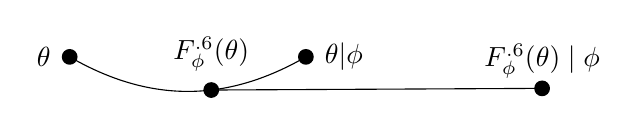
\begin{tikzpicture}
    \coordinate[label=left:$\theta~$] (A) at (0,0);
    \coordinate[label=right:$~\theta|\phi$] (C) at (3,0);
    \coordinate[label=above:$F_\phi^{.6}(\theta)\mid\phi$] (C') at (6,-0.4);
    \draw (A) to[bend right] 
		node[outer sep=0,pos=0.6,label=above:$F_\phi^{.6}(\theta)$](B){} (C);
    \fill 
        (A) circle (0.1)
        (B) circle (0.1)
        (C) circle (0.1)
        (C') circle (0.1);
    \draw (B.center) to (C');
\end{tikzpicture}
\end{center}
% \cref{ax:seq-for-more} also has a more significant effect: it means
\cref{ax:seq-for-more} also ensures
that a high confidence update can be decomposed into
several updates of lower confidence. 


Finally, we impose a mild regularity condition
that can be thought of as
% a special case arising in 
a limit \cref{ax:seq-for-more}
when confidences $\chi_1$ and $\chi_2$ become infinitessimally close;
% for infinitessimal values of confidence (specifically $\chi_1$),
% which we can make sense of because of \cref{ax:diffble}. 
% which we can make sense of via differentiability (\cref{ax:diffble}). 
we make this precise via differentiability (\cref{ax:diffble}). 
% The next axiom states
% This is a relatively minor condition

\begin{CFaxioms}
	\item \label{ax:nopause}
	If
	% $\frac{\partial}{\partial\chi} F(\theta,\chi,\phi) \!=\! 0$
	$\frac{\partial}{\partial\chi} F^\chi_\phi(\theta) = 0$
	and $\chi' > \chi$,
	then 
	% $F(\theta, \chi', \phi) \!=\! \theta$.	 
	$F^{\chi'}_\phi(\theta) = \theta$.	 
\end{CFaxioms}

Intuitively, \cref{ax:nopause} amounts to requiring that updates
do not ``temporarily pause'' for intermediate values of confidence,
and then resume for higher values of confidence.
The culmination of these axioms results in our first definition of an
update function that takes confidence into account.


% For this reason, we give them a special name
% Together, these axioms allow us to define an update rule, by:

\begin{defn}
	A function $F: \Phi \times [0,1] \times \Theta \to \Theta$ 
	satisfying
	\cref{ax:zero,ax:idemp,ax:cont,ax:seq-for-more,ax:diffble,ax:nopause}
	is 
	% an \emph{update function}.
	a \emph{path update function}.
\end{defn}



Path update functions capture some important aspects of uncertain
updating%
---but a number $\chi \in [0,1]$ is not the only useful
way to quantify confidence.
For the full picture of of how these concepts are related, we will
need to look at confidence from several more angles.

% If $\phi_1$ and $\phi_2$ are such that
% $F_{\phi_1}$ and $\phi_2$



% Intuitively,
% \cref{ax:seq-for-more} 
% says that 
